
% to choose your degree
% please un-comment just one of the following
\documentclass[bsc,frontabs,twoside,singlespacing,parskip]{infthesis}     % for BSc, BEng etc.

\usepackage{listings}
\usepackage{color}
\usepackage{hyperref}
\usepackage{paralist}

\usepackage{graphicx}
\usepackage{caption}
\usepackage{subcaption}

% Put page numbers in the middle of the footer
\usepackage{fancyhdr}
\usepackage{titlesec}
\assignpagestyle{\chapter}{fancy}
\pagestyle{fancy}
\fancyhf{} % clear all header and footer fields
\fancyfoot[C]{\thepage}
\renewcommand{\headrulewidth}{0pt}
\renewcommand{\footrulewidth}{0pt}

% Set chapter font
\usepackage{sectsty}
\usepackage[T1]{fontenc}
\usepackage{charter}
\usepackage[expert]{mathdesign}

% Use abstract package and remove abstract from title page
\usepackage{abstract}
\renewcommand{\abstractnamefont}{\normalfont\Huge\bfseries}

% Set chapter font
\chapterfont{\usefont{T1}{bch}{b}{n}\selectfont\huge}

% Set section and subsectionfont
\usepackage{titlesec}
\titleformat{\section}[hang]{
    \usefont{T1}{bch}{b}{n}\selectfont} % "bch" - Bitstream Charter, "b" - bold
    {} % label
    {0em} % horizontal separation between label and title body
    {\hspace{-0.4pt}\Large \thesection\hspace{0.6em}} % code preceding the title
    [] % optional code following the title body
\titleformat{\subsection}[hang]{
    \usefont{T1}{bch}{b}{n}\selectfont} % "bch" - Bitstream Charter, "b" - bold
    {} % label
    {0em} % horizontal separation between label and title body
    {\hspace{-0.4pt}\Large \thesubsection\hspace{0.6em}} % code preceding the title
    [] % optional code following the title body


\definecolor{dkgreen}{rgb}{0,0.6,0}
\definecolor{gray}{rgb}{0.5,0.5,0.5}
\definecolor{mauve}{rgb}{0.58,0,0.82}

\lstdefinelanguage{JavaScript}{
  keywords={break, case, catch, continue, debugger, default, delete, do, else, finally, for, function, if, in, instanceof, new, return, switch, this, throw, try, typeof, var, void, while, with},
  morecomment=[l]{//},
  morecomment=[s]{/*}{*/},
  morestring=[b]',
  morestring=[b]",
  sensitive=true
}

\lstset{frame=tb,
  language=JavaScript,
  aboveskip=3mm,
  belowskip=3mm,
  showstringspaces=false,
  columns=flexible,
  basicstyle={\small\ttfamily},
  numbers=none,
  numberstyle=\tiny\color{gray},
  keywordstyle=\color{blue},
  commentstyle=\color{dkgreen},
  stringstyle=\color{mauve},
  breaklines=true,
  breakatwhitespace=true
  tabsize=2
}


\begin{document}

\begin{titlepage}
    \begin{center}
        \vspace*{1cm}

        \huge
        \textbf{Revision Planner Cross-Platform Web App}

        \vspace{1.5cm}

        \LARGE
        \textbf{Georgi Koshov}

        \vfill

        \Large
        Undergraduate Dissertation\\
        Artificial Intelligence and Computer Science

        \vspace{0.8cm}

        \large
        School of Informatics\\
        University Edinburgh\\
        March 2014

        \vspace{0.8cm}

        
\includegraphics{university}

    \end{center}
\end{titlepage}



\begin{abstract}
	The aim of the project is to develop a working software that has the ability to generate revision schedule for a given list examinable subjects and the corresponding dates. In order to validate the correctness and completeness of the solution, the author has developed a professional-grade web application that has been tested with real users in order to evaluate the qualities, potential and usability of the application.\\

	\centerline{The application is available at:}
	\centerline{\hyperref[http://smartrevise.herokuapp.com/]{http://smartrevise.herokuapp.com/}}
\end{abstract}



%\section*{Acknowledgements}
%Acknowledgements go here.



\tableofcontents

\pagenumbering{arabic}


\chapter{Introduction}

	Revising for exams can be a daunting task. Students often have to prepare for several subjects while going to classes and working on coursework. Furthermore, preparing for a single examination topic involves several phases of study such as revising lecture notes, reading examinable material and revisiting tutorial questions. These tasks, combined with stress and anxiety may lead to lack of concentration, sleep deprivation and total chaos in some extreme cases.

	While computer science does not provide any magic cures for common problems such as short attention spam and lack of interest, the available tools and powerful personal computers make it nearly trivial to design and develop tools that can support students in the chaos called exam revision.

	The objective of this project is to create an application that helps students plan and manage their exam revision. The aim is to make rational assumptions in order to produce a meaningful revision schedule with minimum data. Additionally the application has to allow its users to modify all defaults and let them tailor the results. Finally the goal of this project is to use cutting-edge technologies in order to produce a portable and lightweight app that can be used on desktop PCs as well as on smartphones, thus fitting appealing to a wider range of users and providing useful assistance whenever needed.

	\section{Application overview}

		One of the key aims when designing the application was to produce a result with minimum data required from the user and dynamically visualise the impact of any additional entries or constraints. Therefore students should be able to enter just a list of subjects and their corresponding examination dates, and have a revision schedule generated for them. In addition the produced plan should adhere to the following constraints:

		\begin{compactitem}
		  \item The available revision time is split proportionally between subjects
		  \item No revision is scheduled during exams
		  \item Revision for a given subject should only occur prior to the examination
		  \item No revision is scheduled outside user-definable working hours
		  \item Only one revision event should be scheduled at a given time
		  \item The subtasks of a subject are scheduled in the order entered
		  \item If possible, a subjects are allocated some time every day
		\end{compactitem}

		Additionally users should have the option to enter periods when they are not available or change the relative priorities of subjects and receive immediate feedback in the form of a new revision schedule.

		\subsection{Application portability}

			With the introduction of powerful portable devices that achieve desktop-grade performance in terms of web browsing, it is no longer safe to make assumptions about the screen size or computational resources of the device used to access a web application. Furthermore students are becoming increasingly accustomed to mobile productivity tools and are starting to expect from every modern application a level of accessibility from their smartphones. On top of that, the latest web standards and browser technologies empower developers and provide a good foundation for the rapid creation of portable high-performance applications.

			Therefore this project has been envisioned and implemented with flexibility in mind: all design elements are responsive - the layout adjusts to various screen sizes, while interface elements retain adequate sizes in relation to the input device; the application was built using widely adopted web-standards and can be executed on all modern web browsers on both desktop and mobile applications.

			Ultimately, this approach proved beneficial not only because it allowed rapid prototyping and delivery, but also because it gave the author an excellent insight into continuous delivery, full-stack JavaScript development and valuable knowledge about cutting-edge web technologies.

		\subsection{Solving the scheduling problem}

			Arguably the most critical task for successful completion of the project is developing a correct and efficient scheduling algorithm that is compact enough to be understood and discussed in its entirety. One might be tempted to implement a full-blown constraint satisfaction framework that allows the user to define sets of constraints imposing conditions on variables. A number of search techniques such as backtracking or local search could be used to derive a solution to a system of constraints on a finite domain. However I will argue in Section \ref{algo} that such solution is not required to successfully solve the problem as defined in this report. Furthermore constraint satisfaction algorithms are inherently incomplete, that is an algorithm may solve a problem or prove that it is unsatisfiable, but there are some exceptions when a solution can never be derived. Therefore I have decided to focus on user experience, responsiveness and managed to develop an algorithm that is a fraction of the size of a traditional constraint satisfaction toolkit and is provably correct.

	\section{Success criteria} \label{success_criteria}

		TODO: add some discussion

		The application should:
		\begin{compactitem}
			\item work as intended and as expected
			\item produce realistic and correct revision schedules
			\item provide the same experience on both desktop and mobile devices
			\item give access to the generated schedule from multiple devices
			\item be intuitive and easy to use
			\item be visually appealing and well structured
		\end{compactitem}

	\section{Report Structure}

		The following chapters outline the planning, development and evaluation of the project:

		\begin{compactitem}
			\item Chapter \ref{background} Background provides overview and discussion of similar tools and applications.
			\item In chapter \ref{algo_design} Scheduling Algorithm Design we discuss possible algorithms and describe in detail the solution for the scheduling problem.
			\item Chapter \ref{architecture} Architecture and Implementation includes description of the project's structure and design decisions that were taken during development.
			\item Chapter \ref{evaluation} Evaluation gives arguments in support of the claim that the project was successfully completed.
			\item Chapter \ref{further_work} Further Work outlines useful features that were not implemented but would be good to have and will add to the value of the project.
		\end{compactitem}



\chapter{Background}\label{background}
		In this chapter a brief outline of the available revision planning tools and technology choices will be given.
		In section \ref{apps} we discuss existing software with similar functionality and how that compares to the specification for SmartRevise.


	\section{Existing revision scheduling applications}\label{apps}

		During the project's planning phase a thorough study of the existing applications with related functionality was conducted. The aim was to set realistic goals and success criteria, identify potential pitfalls and justify the need for such application.

		While none of the examined products provided the full set of features - particularly the ability to auto-generate revision schedules - the four applications described below came close to the intended functionality of this project and provided useful insight during the design phase. All applications provide a list or calendar view for examination timetable. Get Revising is the only product that automatically produced a revision plan, while some of the other applications allowed the user the manually add study periods.

		Overall, none of the currently available revision planning applications were suited for students of all ages or study systems, were able to schedule revisions automatically or offered both desktop and mobile presence. These features combined make a strong case for the practicality of the application developed for this project.

		\subsection{ExamTime}
		\textbf{\hyperref[htttp://www.examtime.com/]{htttp://www.examtime.com/}}\\
		ExamTime is the simpler of the two applications. After registering with the service, the user is prompted to add subjects to their dashboard. Subjects are in fact collections of mind maps, quizzes, flash cards and notes, organised under topics.

		There is a calendar view where the user can manually add calendar events for exams, revision sessions or other activities. The application does not allow for the automatic generation of a revision schedule and the user has to complete this activity by themselves.

		\subsection{Get Revising}
		\textbf{\hyperref[http://www.getrevising.co.uk/]{http://www.getrevising.co.uk/}}\\
		Get Revising offers a larger number of features such as Flashcards, Revision Notes, Quizzes, Mind maps and the ability to share resources between students. Some built-in layouts are provided for common GCSE, A Level and University courses that include exam dates and simple content structure for common subjects.

		The user of the study planner feature of Get Revising can set School hours that should be excluded from the revision schedule and the application has the ability to split the time prior to exam dates equally between selected subjects.

		However Get Revising does not allow for a deeper level of detail when it comes to creating a schedule - only events for revising a particular subject can be created, therefore a user cannot include items such as\textit{read textbook, solve tutorials, do past papers, etc.}

		\subsection{S-cool}
		\textbf{\hyperref[http://www.s-cool.co.uk/]{http://www.s-cool.co.uk/}}\\
		S-cool is primarily targeted at high-school students doing GCSE and A Level courses. The web-site requires visitors to create an account before accessing any of its features, prompting for potentially sensible data such as full name, birth date and postcode. Furthermore, a confirmation e-mail was sent immediately following the registration, that contained a plain text record of the password entered in the website.

		Although discussion of the potential security implications caused by these design decisions is beyond the scope of this thesis, security best-practices have been followed while developing this project and further details can be found in section \ref{security} Security.

		After registering, users can create an exam timetable and manually enter multiple revision periods. The simple month view calendar only allows students to enter the date, but not the exact time of events, rather they are displayed as items in a task-list for a given day.

		\subsection{SQA "My Study Plan" and "My Exams" for iPhone}
		\textbf{\hyperref[http://www.sqa.org.uk/sqa/1439.html]{http://www.sqa.org.uk/}}\\
		These two mobile applications were created in conjunction with the Scottish Qualifications Authority to help pupils in secondary school to organise their studies and revision. "My Study Plan" was last updated on 8 April 2011 and does not appear to be actively developed, while "My Exams" is still maintained. The iPhone app is targeted at students in Scottish secondary school and allows them to create exam timetables, add notes to subject areas and share their timetables.

		However, the application lacks integration with desktop tools, while the timetable only allows users to see a list of upcoming exams.

		\subsection{Existing revision scheduling applications - results}
		TODO\\
		- brief discussion of the need for a tool that is not solely targeted at school pupils\\
		- summary of common issues:

		\hspace{10 mm}	- tedious registration process

		\hspace{10 mm}	- lack of portability - the tools are not mobile-friendly

		\hspace{10 mm}	- calendar views are somewhat limited and lack detail

		\hspace{10 mm}	- no notion of instant feedback when changing the parameters of the revision (or lack of such parameters altogether)


	\section{General scheduling and planning applications}
		Note to Paul:
		In your feedback from the Interim report you mentioned that:
		"you probably want to try and say something more general about a wider range of existing work, rather than your more detailed comments on just a couple of application."

		I have selected 5 web applications for project management that are most suitable to the task, i.e. someone can theoretically plan a revision schedule using them. Also according to various sources on the internet, these are currently the best web-based project management tools.

		http://www.gantter.com/ - Free - integrates with Google Docs. A tool for GANTT charts.\\
		http://www.wrike.com/tour/\#getting-things-done - Freemium - a more feature-complete application with mobile apps and collaboration tools.\\
		http://www.aceproject.com/tour/ - Freemium - pretty much the same thing as Wrinkle.\\
		http://office.microsoft.com/en-gb/project/ - Paid - Now part of Office 365, therefore it is technically a web app. Also one of the best project management tools.\\

		My question is whether you meant this by "existing work" or rather algorithms and scheduling techniques, since I will include those in the next chapter?


\chapter{Scheduling Algorithm Design}\label{algo_design}

	- what criteria are you going to allow the user to specify?
	- how did you decide that these are appropriate?
	- discussion of PERT etc and why it might not be a particularly fit
	- mention of constraint-based approaches
	- description of the algorithm that you finally used

	In Section \ref{scheduling} the reader may find a high-level summary of existing project-management techniques and some arguments about their applicability in the current project.

	Due to the advancement of faster, more powerful web-browsers, featuring robust engines for running efficiently large amounts of  code and with the continuous effort by organisations such as Mozilla and Chromium to drive web standards further and develop powerful open-source technologies for the next generation of Web, it is no longer infeasible to develop an entire application stack using a single programming language - ECMAScript, or more commonly known as JavaScript.

	Some of the arguments in support of such design decision include the ability to exchange JavaScript objects between server and client without having to convert them during transport, being able to plug community libraries at all levels of the project without having to worry about compatibility or portability, but most of all due to the sheer convenience of having an entire application stack built with the exact same tools and following the same design philosophy.

	A more traditional way to solve the problem defined in this report would be to create a server-centric application that relies on technologies such as PHP, Python or Java to do the majority of the work on the server and send the rendered HTML templates as static files to the client. While this solution is widely used in practice, recent years have seen a change in the web application design approach, targeted at thinner back-ends and outsourcing the majority of the application logic to the user's browser.

	\section{Discussion of scheduling methods}\label{scheduling}

		Several options for scheduling of concurrent events exist in the project-management domain. Critical Path Method and Program Evaluation and Review Technique are the two most widely used techniques for solving a project-management problem. This section will include a brief overview of the two techniques as well as some discussion of the applicability of CPM and PERT for the current problem.

			\subsection{Critical Path Method}

			\subsection{Program Evaluation and Review Technique}

			\subsection{Constraint satisfaction}

		Traditionally CPM and PERT are used when solving problems where a number of resources have to be shared between many possibly concurrent tasks. Example scenarios include organising receptions and events where many workers need to complete several tasks that could include some dependencies.

		The problem that SmartRevise is attempting to solve assumes that a single worker - the student - needs to decide on a suitable ordering and allocation of several streams of independent tasks. There is no notion of event overlap - at any given point the student is revising a single subject. Additionally we assume that one subject does not depend on another since all courses are deemed self-contained. Therefore the scheduling algorithm needs to track only dependencies of the form: Read textbook for subject X $\rightarrow$ Solve tutorial questions for subject X $\rightarrow$ Attempt past papers for subject X $\rightarrow$ Do exam of subject X. Therefore neither CPM nor PERT are directly applicable in this case. However, when determining the critical path a typical CPM implementation walks the network diagram of a scheduling problem forwards and backwards. A similar approach will be outlined on Section \ref{algo} when efficiently deciding on a suitable partitioning of the available time.



	\section{SmartRevise algorithm}\label{algo}

		The algorithm that was developed for SmartRevise revision scheduling solves the problem on incompleteness, typically associated with constraint satisfaction, by limiting the domain and introducing a single relaxed constraint - amount of hours spent on each subject. The algorithm successfully finds schedules that are intuitively correct and runs efficiently without any noticeable delays. Most of all, the entire scheduling software is executed in the user's browser, which makes the application self-contained and less reliant on a centralised server with high performance.

		The SmartRevise algorithm takes the following input arguments:

		\begin{description}
			\item[Exams] \hfill \\
				An array of \textbf{Exam} objects. Each object has the following attributes: \\
				\textit{Title} - name of subject\\
				\textit{Date} - date and hour of examination\\
				\textit{Duration} - duration of examination\\
				\textit{Portion} - a floating point number [0,1], the relative portion of revision time that will be spent on subject\\
				\textit{Components} - sub-tasks that need be completed as part of the revision for the subject
			\item[Revision start] \hfill \\
				Usually the current time
			\item[Daily start and end time] \hfill \\
				Used to define waking hours available for revision, e.g. 9AM - 6PM
			\item[Additional blocking events] \textit{optional} \hfill \\
				Events that indicate a period when the student is not available
		\end{description}

		The pseudo-code outlined in Listing \ref{algoCode} presents the basic structure of the SmartRevise scheduling algorithm:

		\begin{lstlisting}[caption="SmartRevise scheduling algorithm", label=algoCode]
Exams.sort(exam.date, ascending);
var revisionEnd = Exams[exams.length - 1];
var revisionLength = difference(revisionStart, revisionEnd);

// Divide revision period in "chunks" of time between exams
// Examine days in reverse order starting from last day
for (var day=revisionLength; day>0; day--) {
	if (day.hasNoExams) {
		currentChunk.slices.push( day );
	} else {
		currentChunk.slices.push( period(exam.date+exam.duration, day.end) );
		currentChunk = new Chunk
	}
}

// Calculate total revision time
var revisionTime;
for (chunk in chunks) {
	for (slice in chunk.slices) {
		revisionTime += chunk.length;
	}
}

// Determine revision time per subject
for (exam in exams) {
	exam.time = revisionTime * exam.portion;
}

// Starting from last chunk proportionally (to remaining hours of each subject) split time between exams, keeping track of spent hours
var events = [];
for (chunk in chunks.reverse) {
	for (slice in chunk.slices){
		// Determine the total remaining revision time for the exams remaining after the current chunk
		var chunkExamsTime;
		for (exam in chunk.exams) {
			chunkExamsTime += exam.time;
		}

		// Allocate proportional amount of time to each exam
		for (exam in chunk.exams) {
			var subjectTime = (exam.time / chunkExamsTime) * slice.length;
			exam.time -= subjectTime;
			// Create new revision event and add it to the list of events
			events.push(new SubjectRevision(exam.title, subjectTime));
		}
	}
}

		\end{lstlisting}


		Each Chunk object contains several Slices - an uninterrupted working time, e.g. 31/06/2014 09:00 - 31/06/2014 18:00. A chunk also has an Exams attribute that contains an array of Exam objects with due date after the end of the chunk. Therefore the first chunk contains all slices from the start of the revision until the first exam date. Additionally $ Chunk[0].exams $ contains all exams in the schedule.

		Using the logic outlined in the pseudo-code in Listing \ref{algoCode} and by including edge-case handling and means for converting and executing mathematic expressions on JavaScript Date objects, a JavaScript method was developed that can successfully partition the period between a given start date and a number of random exam dates.

		One notable exception surfaced during the development of the algorithm - if an exam is scheduled at the very beginning of a lengthy exam diet it might be the case that there is not enough time between the revision start and the exam date to spend the total time allocated for that subject. Despite that, such subjects are allocated most of the available time and without adding any specific handling for such cases, the algorithm produces sensible and meaningful revision schedules.




\chapter{Architecture and Implementation}\label{architecture}

	- choice of tools and justification
	- RWD

	\section{Project architecture}

		SmartRevise is a client-side JavaScript application based on the Google AngularJS framework that is served by a NodeJS server. The entire application is downloaded by the client upon establishing connection with the server and the user's browser is responsible for rendering views and navigating between them. A similar approach is used by Google for their Gmail application and it allows for offloading the rendering responsibility from the server to the client. Additionally, after downloading the application, the only data that is exchanged with the server is in the form of JavaScript objects. Since the front-end can be cached by the browser, this solution can decrease traffic and improve the user's experience. On the other hand, since all further server requests are executed via an API to the database, it is trivial to implement memory caching, load-balancing and advanced protection to the leaner and less complicated back-end.

		Application deployment, provisioning of the environment and dependency management is also handled by JavaScript services such as Grunt and Bower. Further details about configuring and using those can be found in section \ref{tools}.

	\section{Client-side application}

		The front-end of SmartRevise was built using AngularJS. This is a front-end web application framework built by engineers at Google, aiming for rapid development of lightweight yet powerful browser applications. It follows the $ Model-View-Controller [MVC] $ philosophy and allows the developer to built modular applications by allowing the abstraction of every single interface element or piece of functionality in an Angular structure called Directive. A directive could be anything from a simple UI element with additional features, to complex scheduling algorithms that can be packaged and distributed with ease.

		There are alternatives to Angular such as EmberJS, Knockout and Backbone. The decision to use Angular was made in an effort to extend the author's knowledge of JavaScript MVC frameworks and due to the abundance of resources about the software on the Internet.

	\section{Server and REST API}

		The back-end of the application was built using NodeJS. This is a JavaScript platform built on Google Chrome's JavaScript V8 engine. It is a lightweight event-driven framework that aids the building of scalable and efficient server application.

		Routing, request handling and connection to the database is achieved using Express - a JavaScript framework for building web applications based on Node. The purpose of the library is to provide basic functionality such as authentication, user sessions and request serialisation out of the box.

		The database was built using MongoDB. This is a mature open-source NoSQL database written in C++ that provides excellent interfaces for data exchange with Node application. Mongo features an SQL-like query language based on JavaScript and allows the developer to store entire JavaScript objects without having to convert back and forth to a relational schema. NoSQL solutions are not optimal for performance-centric applications or solutions involving massive amounts of data. In the case of SmartRevise there are several arguments in support of such design decision:

		\begin{description}
			\item[Rapid development] \hfill \\
				Changes in the database schema are largely effortless since there is no need to convert JavaScript objects to tuples in a relational database
			\item[One lookup and update per user session] \hfill \\
				Since SmartRevise is a client-side application, all changes to the data are made in the user's browser and stored locally until the end of the interaction. Therefore the number of database lookups is kept minimal
			\item[Ability to switch database engine at any point] \hfill \\
				The above items outline MongoDB's advantages during development. Since all data calls are routed via an API, it would be trivial to switch MongoDB with a traditional SQL database and develop adapters that convert SQL relations to the corresponding JavaScript objects. Currently there is no need for higher performance, but should any issues emerge that cannot be solved by the MongoDB community, the architecture allows for quick exchange of components.
		\end{description}


	\section{Security}\label{security}
	TODO
	Sessions, salted hash passwords, no SSL

	\section{Additional tools}\label{tools}

		This section will provide a review of the miscellaneous software packages that were used in order to ease development, improve the quality of the software and simulate as closely as possible a real production environment.

		\subsection{Grunt}
			Grunt is a JavaScript Task Runner. It allows the developer to automate repetitive tasks by defining a Gruntfile.js with automation parameters. The biggest advantage of Grunt over similar technologies such as Puppet or Chef is its growing environment focused on JavaScripts.

			In the setup for SmartRevise, Grunt is used to compile multiple JavaScript libraries to a single script file, compress the code using best practices in order to achieve faster and smoother experience for the user, run the database and server applications as well as monitor the project directory for file writes and automatically recompile the application.

			Additionally using Grunt one can generate templates for various Angular components such as new routes, templates or directives, as well as export a compiled version of the application that can be published to a SaaS provider such as Heroku in less than a minute.

			In summary, Grunt is a crucial component in every professional toolkit nowadays and helps deliver ideas very quickly without technology getting in the way.

		\subsection{Bower}
			Bower is the first JavaScript package manager for front-end web projects. It makes downloading and managing a large number of external dependencies effortless compared to manual management of libraries.

			Package management is traditionally considered a trivial problem for modern software engineering, but since the majority of JavaScript tools are relatively young and less developed, being able to manage the entire stack of a web application with ease and convenience is a significant step forwards that makes this project better suited for future development.




\chapter{Evaluation}\label{evaluation}

	Chapter \ref{evaluation} describes the actions that were taken in order to evaluate the SmartRevise scheduling application.

	The chapter includes discussion of four aspects of the evaluation: correctness of the scheduling algorithm in section \ref{algo_eval}; usability testing and user feedback in section \ref{user_eval}; experiments related to portability and accessibility of the responsive design in section \ref{portability_eval}, and overall performance metrics of the production environment in section \ref{prod_eval}.

	The purpose of this chapter is to assess the applications against the goals that were defined at the beginning of the project, i.e. the application should:
	\begin{compactitem}
		\item work as intended and as expected
		\item produce realistic and correct revision schedules
		\item provide the same experience on both desktop and mobile devices
		\item give access to the generated schedule from multiple devices
		\item be intuitive and easy to use
		\item be visually appealing and well structured
	\end{compactitem}

	With the support of these arguments I will argue that the task was successfully completed and adheres to high professional standards.

	\section{Unit testing of algorithm}\label{algo_eval}

		The most immediate form of validation for the core functionality of the SmartRevise revision planner was the development of unit tests that check the output of the scheduling algorithm against some basic correctness criteria:

		\begin{compactitem}
		  \item The available revision time should be split proportionally between subjects
		  \item Revision for a given subject should only occur prior to the examination
		  \item No revision should be scheduled during exams
		  \item No revision should be scheduled outside user-definable working hours
		  \item Only one revision event should be scheduled at a given time
		  \item The subtasks of a subject are scheduled in the order entered
		  \item If possible, all subjects are allocated revision time every day
		\end{compactitem}

		A core part of the application stack that was used to create SmartRevise is a unit testing framework that allows the development of both functional and interface tests for all components of the application. The project setup allows automatic generation of test scripts for all application components generated by the Yeoman recipes (see chapter \ref{architecture} Architecture and Implementation). This means that the developer is encouraged to employ a Test Driven Design pattern and define some basic correctness criteria before actually implementing the components of the system.

		During the development of SmartRevise, I decided to use these facilities while extending the scheduling algorithm. This was inspired by the involuntary introduction of several regressions after adding features to the initial algorithm. After I added the tests described below, the unit tests were ran before each deployment to the application host which guaranteed that the application will not be broken by a subtle change in the code.

		All algorithm unit tests use the same pseudo data of 5 exams situated 10 days ahead of the current date, over the span of 5 days. The reason to choose exam dates on a fixed point in the future is to guarantee that the tests are deterministic and negative test results can be replicated.

		\subsection{Revision for a given subject should only occur prior to the examination}
		The first unit test examines whether all revision sessions for a given subject are scheduled before the corresponding exam:

		\begin{lstlisting}
it('all revision events for a given exam should end before the exam\'s date', function () {
  // Run algorithm
  scope.runAlgorithm({newData: true, fromCache: true});

  var correct = true;
  for (var i = 0; i < scope.exams.length; i++) {
    var title = scope.exams[i].title;
    for (var j = 0; j < scope.calendarEvents.length; j++) {
      if (// select revision events for this exam
          scope.calendarEvents[j].title.indexOf(title) != -1 &&
          // make sure this is not the exam itself
          scope.calendarEvents[j].title !== scope.exams[i].title &&
          // check if the revision precedes the exam (time diff is >= 0)
          scope.exams[i].date.diff(moment(scope.calendarEvents[j].start)) < 0 &&
          scope.exams[i].date.diff(moment(scope.calendarEvents[j].end)) < 0
          ) {
        correct = false;
      }
    };
  };
  expect(correct).toBe(true);
});
		\end{lstlisting}

		If the scenario comes across a calendar event whose title suggests that it belongs to the revision of a subject, whose exam is over, the test case fails.

		\subsection{Events in the schedule should not overlap}
		The second test case ensures that no two events in the algorithm output overlap.

		\begin{lstlisting}
it('events in the schedule do not overlap', function () {
  // Run algorithm
  scope.runAlgorithm({newData: true, fromCache: true});

  var correct = true;
  for (var i = 0; i < scope.calendarEvents.length; i++) {
    var event_start = moment(scope.calendarEvents[i].start);
    var event_end = moment(scope.calendarEvents[i].end);
    for (var j = 0; j < scope.calendarEvents.length; j++) {
      var other_start = moment(scope.calendarEvents[j].start);
      var other_end = moment(scope.calendarEvents[j].end);
      // make sure we are not checking against the same event
      if (j !== i) {
        if (// event J starts before event I and they overlap
            (event_start.diff(other_start) >= 0 && event_start.diff(other_end) < 0) ||
            // event J starts after event I and they overlap
            (event_start.diff(other_start) < 0 && event_end.diff(other_start) > 0)) {
          console.log(scope.calendarEvents[i], scope.calendarEvents[j]);
          correct = false;
        }
      }
    };

  };
  expect(correct).toBe(true);
});
		\end{lstlisting}

		In this case the JavaScript Date Objects are manipulated using the MomentJS library in order to find the absolute difference between the start and end dates of every pair of events in the output schedule. If an illegal overlap is detected, the test fails.

		\subsection{No revision should be scheduled outside user-definable working hours}
		The last two tests follow a similar structure and check that no revision events are scheduled outside of the default revision times - 9AM to 6PM.

		\begin{lstlisting}
it('all revision events should begin after the daily start time - 9AM by default', function () {
  // Run algorithm
  scope.runAlgorithm({newData: true, fromCache: true});

  var correct = true;
  for (var i = 0; i < scope.calendarEvents.length; i++) {
    // Check if this is a revision event, not an exam (exams could be any time)
    if (scope.calendarEvents[i].title.indexOf('revision') !== -1) {
      if (moment(scope.calendarEvents[i].start).hour() < 9) {
        correct = false;
      }
    }
  };
  expect(correct).toBe(true);
});

it('all revision events should end before the daily end time - 6PM by default', function () {
  // Run algorithm
  scope.runAlgorithm({newData: true, fromCache: true});

  var correct = true;
  for (var i = 0; i < scope.calendarEvents.length; i++) {
    // Check if this is a revision event, not an exam (exams could be any time)
    if (scope.calendarEvents[i].title.indexOf('revision') !== -1) {
      if (moment(scope.calendarEvents[i].end).hour() > 18) {
        correct = false;
      }
    }
  };
  expect(correct).toBe(true);
});
		\end{lstlisting}

		\subsection{Unit testing summary}
		Using the set of tests I was able to identify a bug which caused revision events to be scheduled beyond the pre-defined working times. This issue was occurring because exams can have arbitrary starting times but initially I had not taken this into account while dividing the free time between exams into revision "slices".

		Overall unit tests helped identify some weaknesses in the design of the algorithm and prevented the pushing of bugs to the live environment. The test scenarios described above cover the more subtle aspects of the scheduling algorithm, while requirements such as the proportional distribution of time were omitted since those were either guaranteed by the core logic of the scheduling algorithm or were inherently non-deterministic due to the varying time availability, e.g. if a user enters two exams - the first in one week, the second in a few months - it would be impossible to split the available revision time equally without penalising one of the subjects.

		As a final note it is worth mentioning that it would be trivial to define a Git pre-commit hook that runs all unit tests prior to pushing changes in the source code. In case a richer set of tests is used, this can prevent poorly planned or executed code changes from breaking the live environment of the application.


	\section{Evaluate usability of application}\label{user_eval}

		Arguably the biggest challenge is developing a visually appealing, intuitive user interface that suits the needs of test users and can provide some value if added to a student's workflow.

		Unfortunately testing the finished application in a real exam setting would be impossible before the deadline of this project, but the author intends to evaluate the application extensively with fellow students in order to identify potential sources of confusion, any shortcomings or inconsistency. However there are few well-studied methods for formally evaluating user experience, therefore the main form of evaluation will be verbal feedback and observation.

		\subsection{Preliminary usability testing}

		\subsection{Feedback from final version}


	\section{Portability and accessibility}\label{portability_eval}

		\subsection{Mobile performance}


		\subsection{Responsive web design}

			\begin{figure}
			        \centering
			        \begin{subfigure}[b]{0.5\textwidth}
			                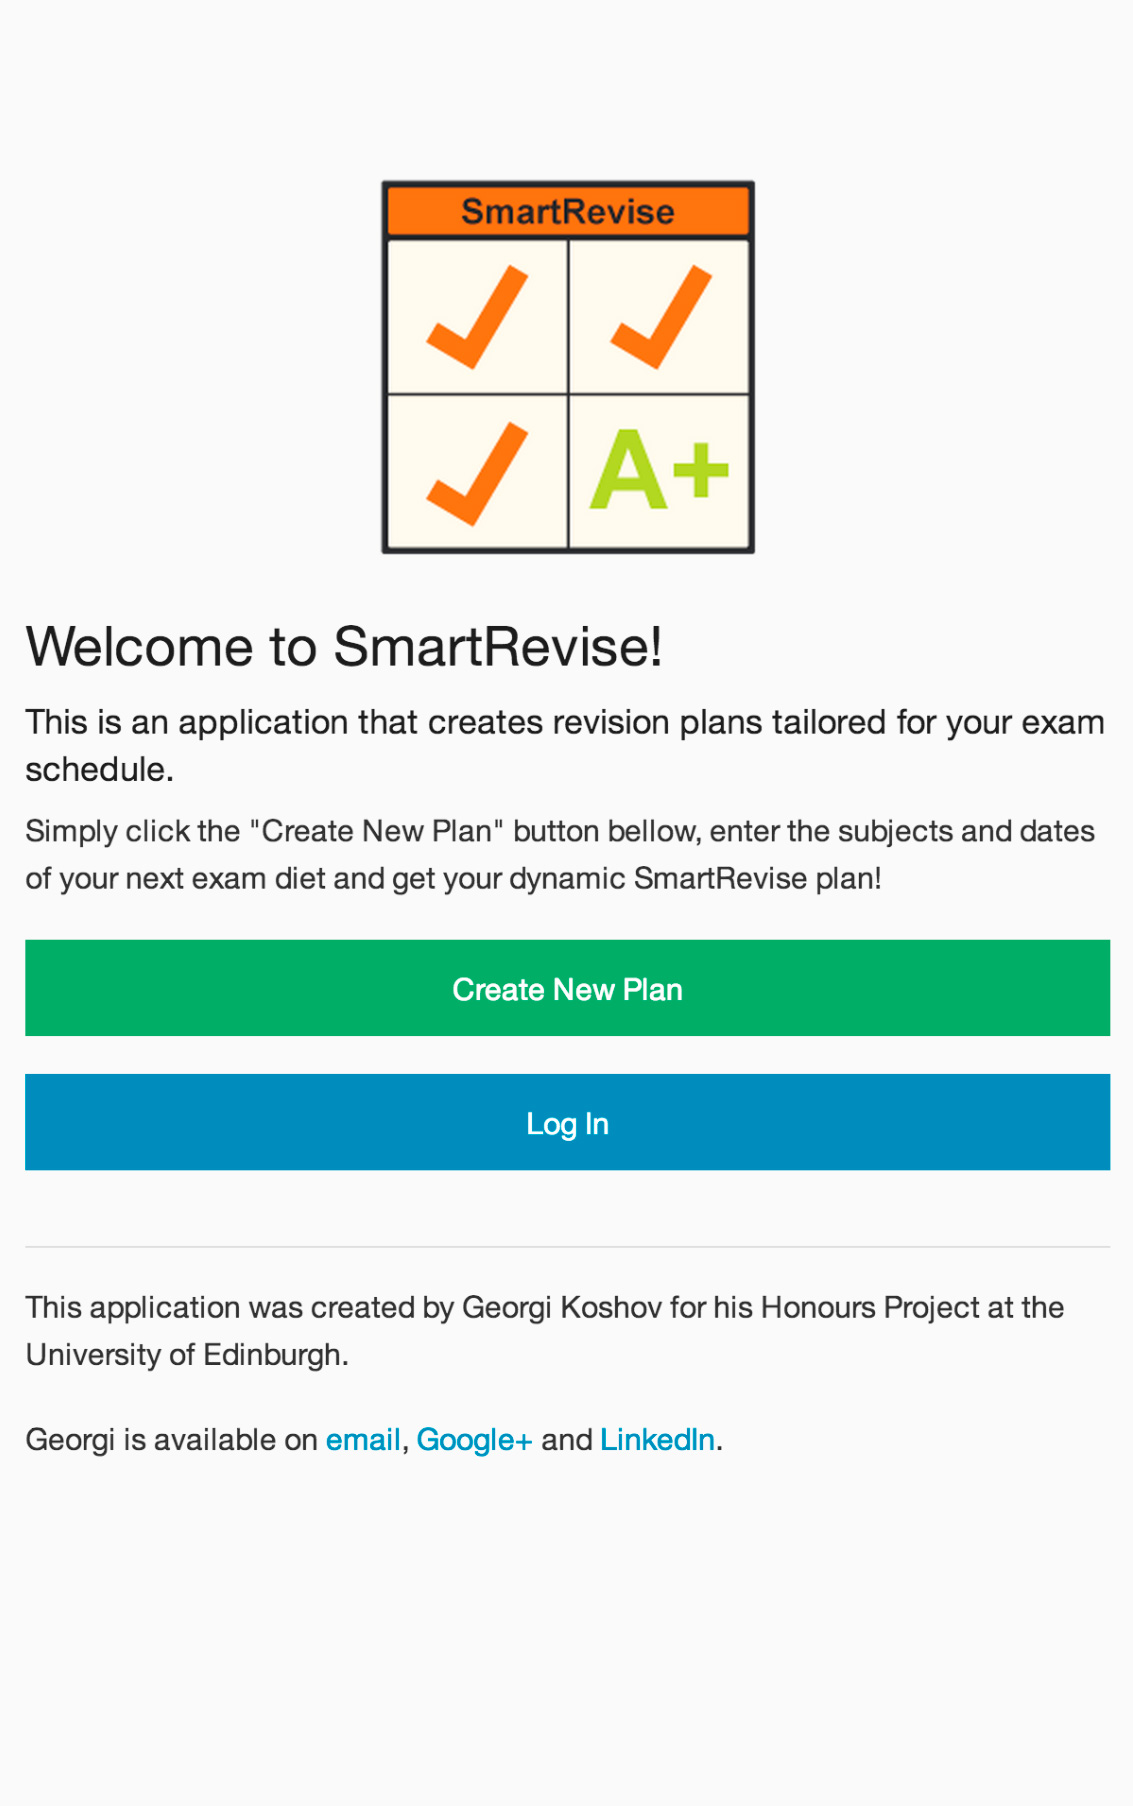
\includegraphics[width=\textwidth]{home}
			                \caption{Home page}
			                \label{fig:home}
			        \end{subfigure}%
			        ~ %add desired spacing between images, e. g. ~, \quad, \qquad etc.
			          %(or a blank line to force the subfigure onto a new line)
			        \begin{subfigure}[b]{0.5\textwidth}
			                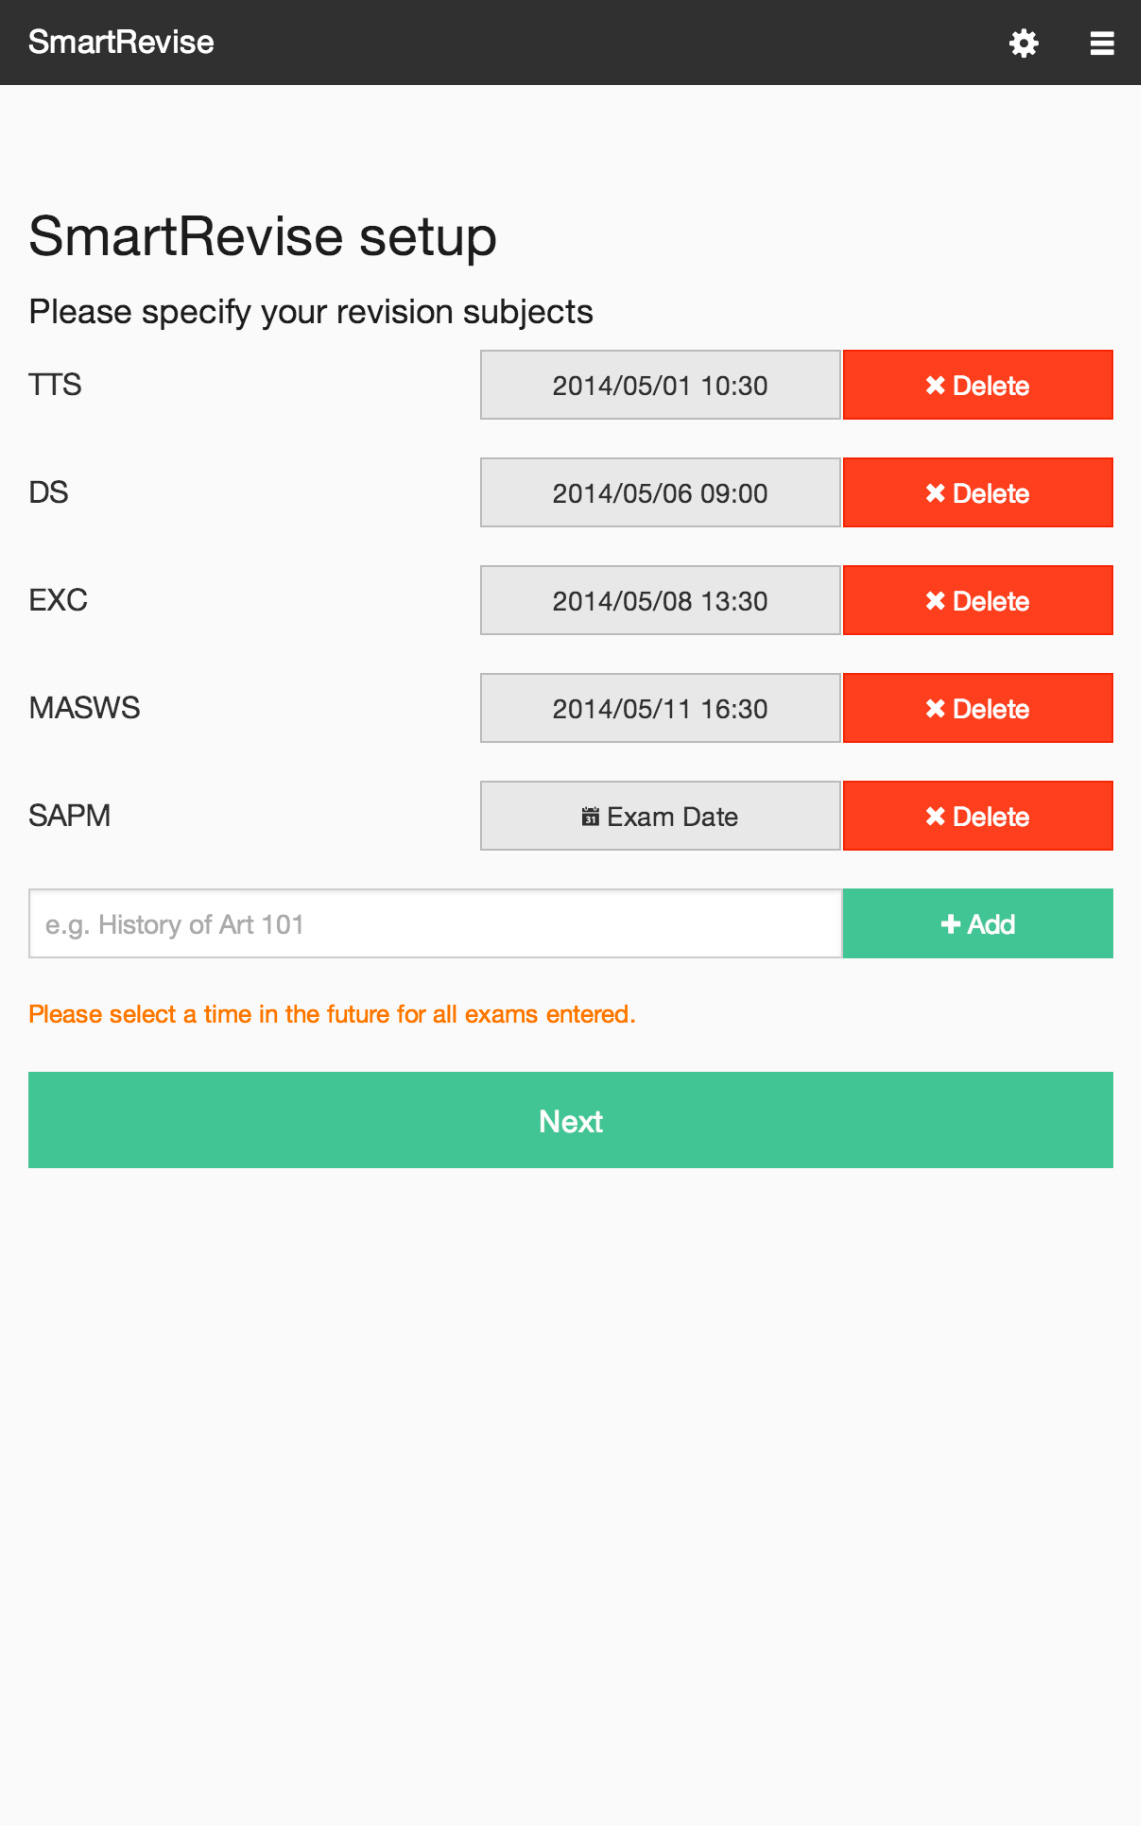
\includegraphics[width=\textwidth]{setup}
			                \caption{Setup page}
			                \label{fig:setup}
			        \end{subfigure}
			        \caption{SmartRevise on Nexus 7 tablet - 800px by 1280px}\label{fig:setup_and_home}
			\end{figure}

			\begin{figure}[p]
			    \centering
				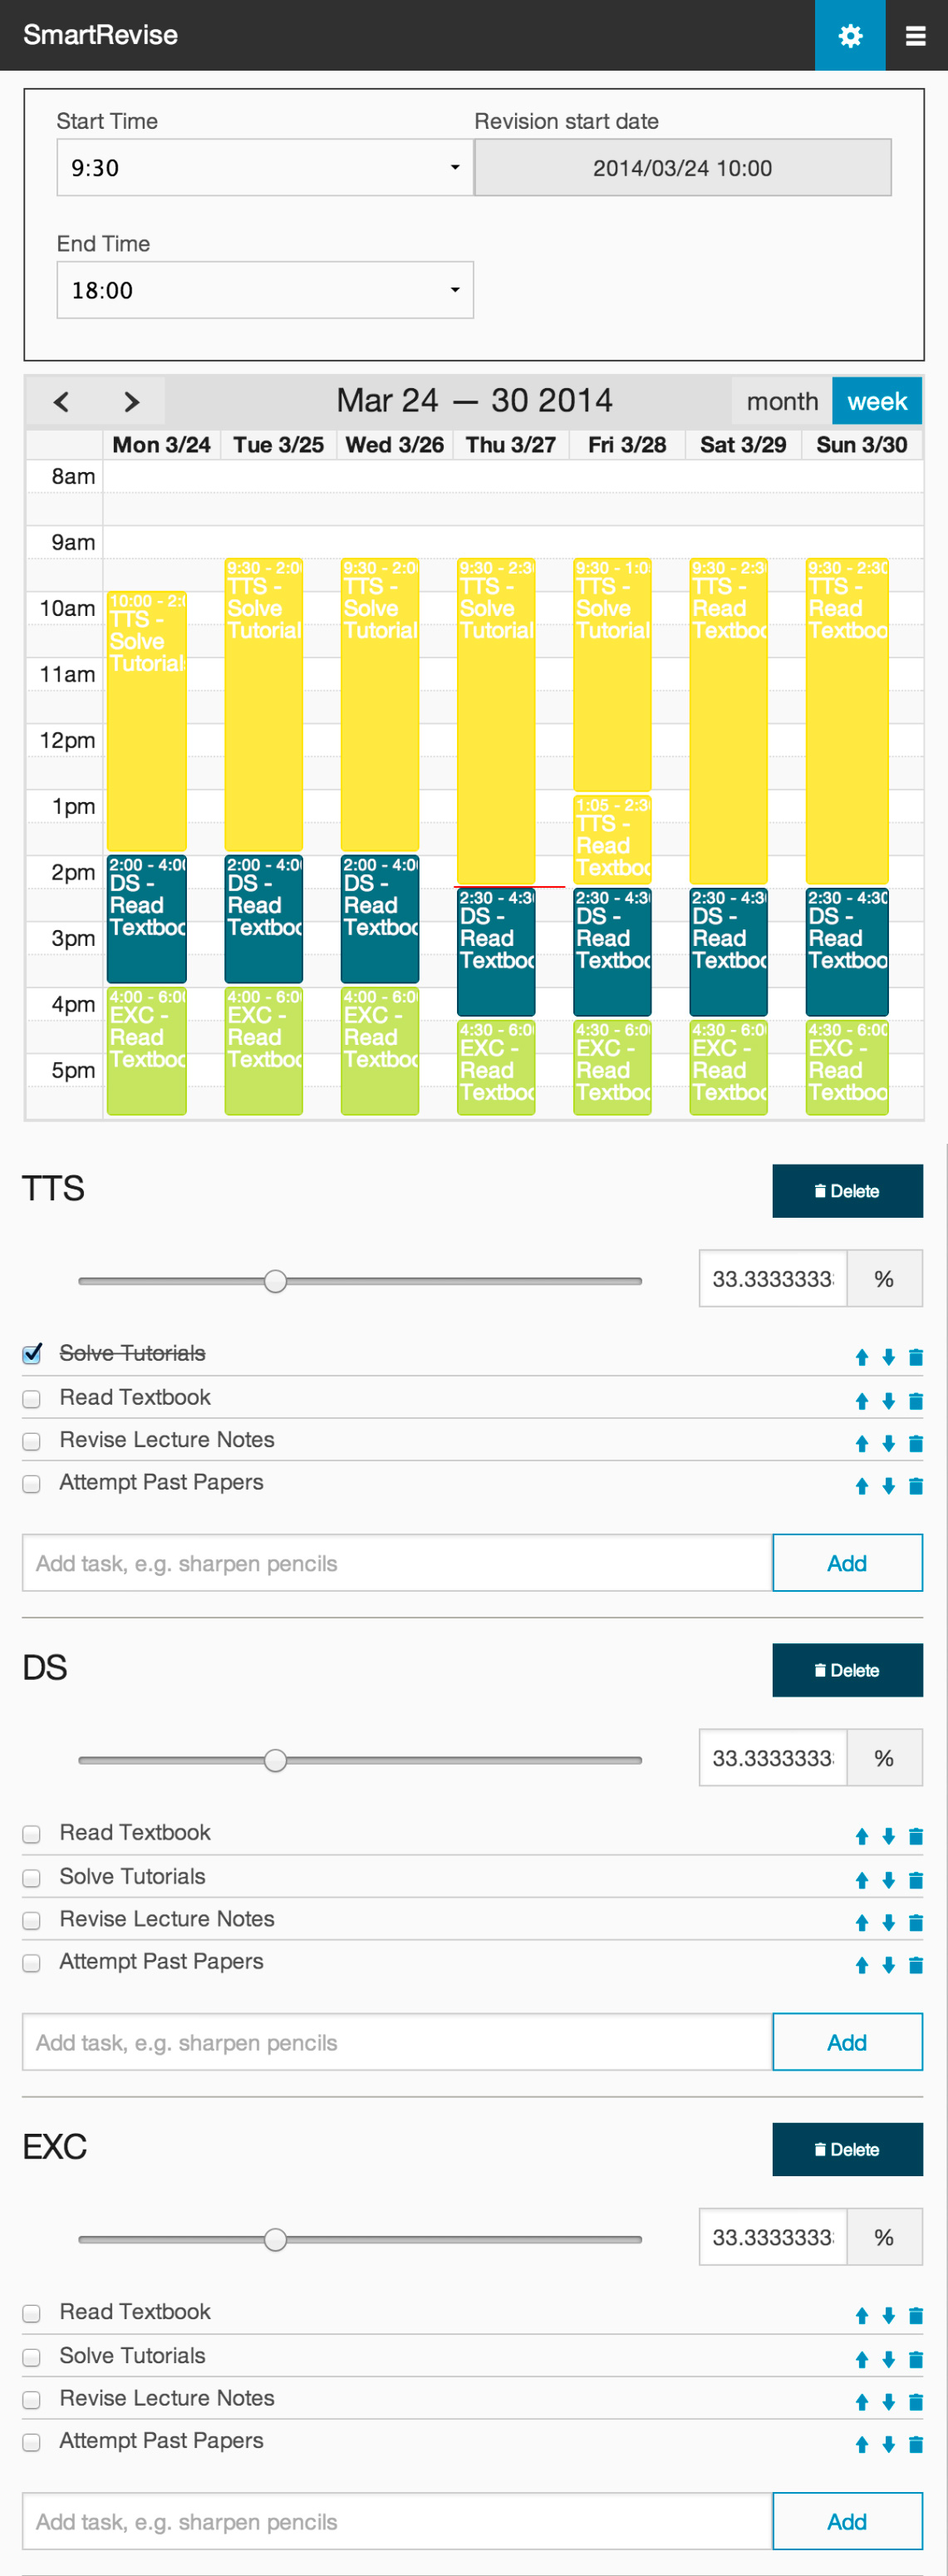
\includegraphics[height=\textheight]{result}
			    \caption{Generated revision plan}
			    \label{fig:result}
			\end{figure}

			\begin{figure}
			        \centering
			        \begin{subfigure}[b]{\textwidth}
						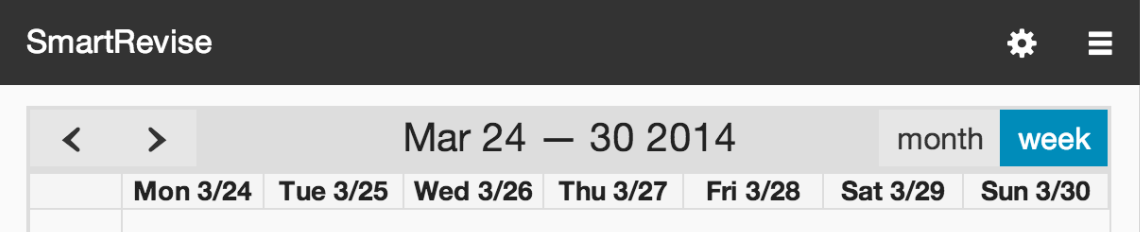
\includegraphics[width=\linewidth]{result_menu_collapsed}
					    \caption{Navigation bar on mobile devices - collapsed}
					    \label{fig:result_menu_mobile}
			        \end{subfigure}

	                \begin{subfigure}[b]{\textwidth}
	        			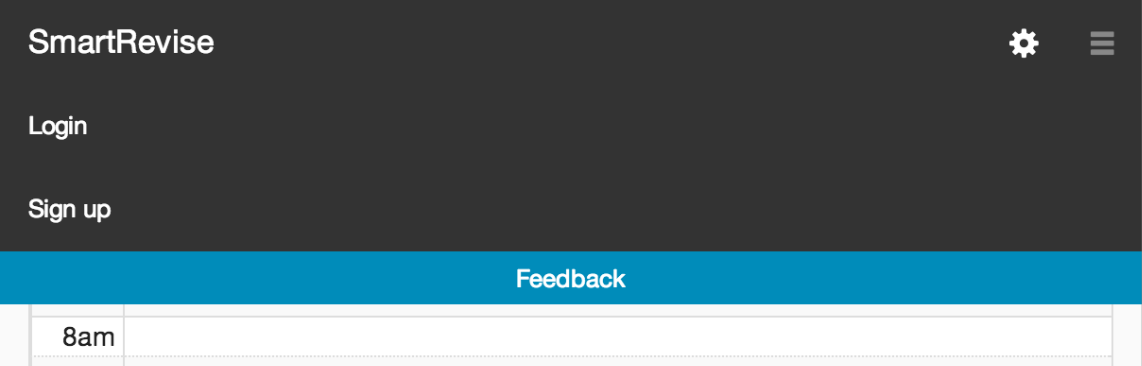
\includegraphics[width=\linewidth]{result_menu_expanded}
	        		    \caption{Navigation bar on mobile devices - expanded}
	        		    \label{fig:result_menu_mobile}
	                \end{subfigure}

			        \begin{subfigure}[b]{\textwidth}
						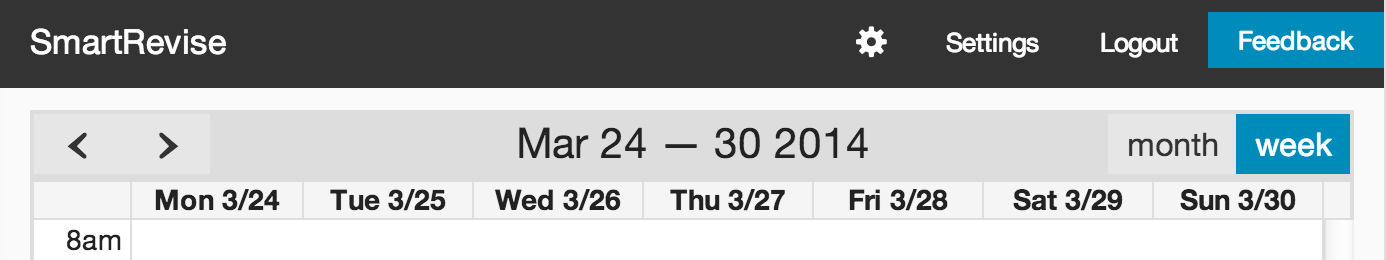
\includegraphics[width=\linewidth]{result_menu_normal}
					    \caption{Navigation bar on large screens (wider than 640px)}
					    \label{fig:result_menu_desktop}
			        \end{subfigure}
			        \caption{Navigation bar}\label{fig:navbar}
			\end{figure}


		\subsection{Accessibility}

			em units - good for higher DPI and devices for disabled people

			semantic markup



	\section{Performance in production environment}\label{prod_eval}

		NewRelic uptime and JavaScript strict mode

		No previous experience with live systems of larger and no exposure to the implications of high availability systems.

		Peak of 100 server requests per minute - which could bring down a poorly optimized app on a small gear. - talk about Heroku...




\chapter{Further work}\label{further_work}

	\section{Integration with existing organisation tools}

		A lot of students use free tools such as Google Calendar or Apple Calendar to organise their schedules and have the information served to all digital devices they use. Google provides an API for developing applications using Calendar's infrastructure and the set up process required for a user to connect their Google Calendar with an external application is mostly effortless and arguably intuitive. Therefore on of the design goals for SmartRevise would be integration with Google's Calendar API and adding support for exporting the generated calendar events to a User's calendar. Additionally, creating a calendar experience within SmartRevise that resembles Google's will make the user's interaction less difficult and considerably more intuitive.

		\textbf{NOTE} Google Calendar has not been integrated with the application, although the calendar view is visually similar to Google Calendar and several of the features were inspired by it. Should I include this as a good to have/future work?




\chapter{Conclusion}

	As indicated in this report, the author has studied the applications that advertise similar functionality to the one intended by the project specification. Applicable algorithms and scheduling techniques have been studied and significant progress has been achieved in developing a working implementation of the outlined architecture.

	Overall the project is on schedule and the application appears to meet the design goals of the given specification.



% use the following and \cite{} as above if you use BibTeX
% otherwise generate bibtem entries
%\bibliographystyle{plain}
%\bibliography{mybibfile}


\end{document}
